%GiG
\documentclass{beamer} 
\usetheme{Copenhagen}
\setbeamertemplate{navigation symbols}{}
\setbeamertemplate{headline}{}
\DeclareMathOperator*{\argmax}{arg\,max}

\usepackage{hyperref}


\definecolor{azure}{rgb}{0.0, 0.5, 1.0}
%\newcommand{\tblue}[1]{\textcolor{blue}{#1}}
\newcommand{\tblue}[1]{{\Large {\textcolor{azure}{#1}}}}
\newcommand{\thblue}[1]{{\Huge {\textcolor{azure}{#1}}}}
\newcommand{\hred}[1]{{\textcolor{red}{#1}}}
\newcommand{\furl}[1]{{\footnote{\url{#1}}}}

\newcommand{\mypause}{\pause}
%\newcommand{\mypause}{}

\title[Saravanan Thirumuruganathan] 
{Lecture 8: Regression Trees}

\author[CSE 5334] 
{Instructor: Saravanan Thirumuruganathan}

\date[] 

\begin{document}


\begin{frame}
  \titlepage
\end{frame}

%\begin{frame}{Outline}
%  \tableofcontents
%  % You might wish to add the option [pausesections]
%\end{frame}

\section{Outline}

\begin{frame}
\frametitle {Outline}
    \begin{enumerate}
        \item Regression
        \item Linear Regression
        \item Regression Trees
    \end{enumerate}
\end{frame}


%\begin{frame}{In-Class Quizzes}
%\begin{itemize}
%\item {\Large {\bf URL:}} {\LARGE \bf \url{http://m.socrative.com/}} 
%\item {\Large {\bf Room Name:} {\LARGE \bf 4f2bb99e}}
%\end{itemize}
%\end{frame}


\section{Regression}
\begin{frame}{} 
    \begin{center}
        \thblue{Regression and Linear Regression}
    \end{center}
\end{frame}

\begin{frame}{Supervised Learning}
    \begin{itemize} 
        \item {\bf Dataset:}
        \begin{itemize}
            \item \hred{Training} (labeled) data: $D = \{ (x_i, y_i) \}$
            \item $x_i \in \mathbb{R}^d$
            \item \hred{Test} (unlabeled) data: $x_0 \in \mathbb{R}^d$  
        \end{itemize} 
        \item {\bf Tasks:}
        \begin{itemize}  
            \item Classification: $y_i \in \{1, 2, \ldots, C\}$ 
            \item Regression: $y_i \in \mathbb{R}$
        \end{itemize}
        \item {\bf Objective:} Given $x_0$, predict $y_0$
        \item {\bf Supervised} learning as $y_i$ was given during training
    \end{itemize} 
\end{frame}

\begin{frame}{Regression}
    \begin{itemize}
        \item Predict cost of house from details
        \item Predict job salary from job description
        \item Predict SAT, GRE scores
        \item Predict future price of Petrol from past prices
        \item Predict future GDP of a country, valuation of a company
    \end{itemize}
\end{frame}

\begin{frame}{Linear Regression : One-dimensional Case}
    \begin{center}
        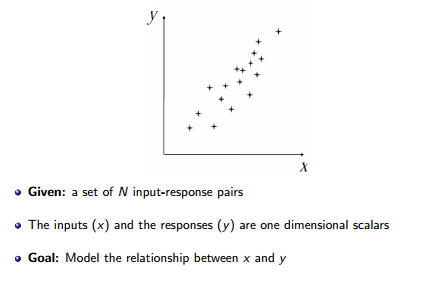
\includegraphics[scale=0.6]{linearRegr1D1.png}
    \end{center}
\end{frame}
\begin{frame}{Linear Regression : One-dimensional Case}
    \begin{center}
        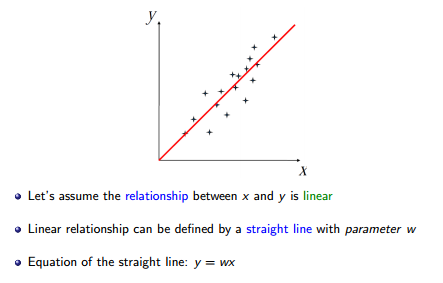
\includegraphics[scale=0.6]{linearRegr1D2.png}
    \end{center}
\end{frame}
\begin{frame}{Linear Regression : One-dimensional Case}
    \begin{center}
        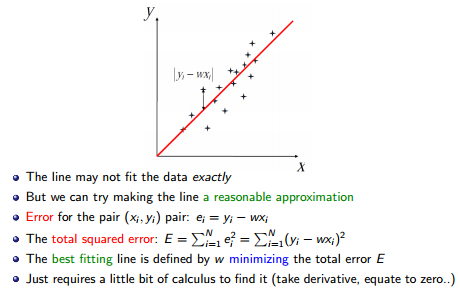
\includegraphics[scale=0.6]{linearRegr1D3.png}
    \end{center}
\end{frame}


\begin{frame}{Linear Regression: Poverty vs HS Graduation Rate}
    \begin{center}
        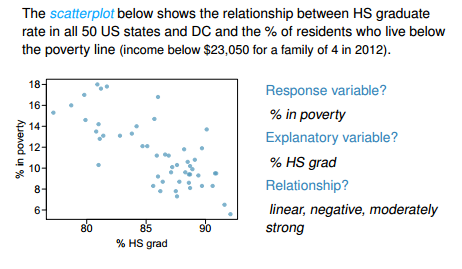
\includegraphics[scale=0.6]{povertyVsHSGradRate1.png}
    \end{center}
\end{frame}
\begin{frame}{Linear Regression: Poverty vs HS Graduation Rate}
    \begin{center}
        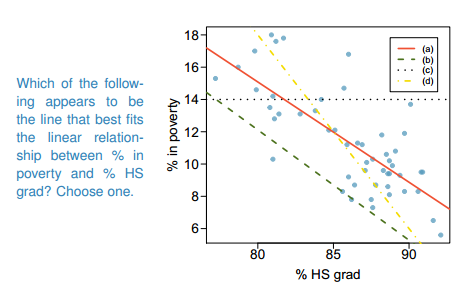
\includegraphics[scale=0.6]{povertyVsHSGradRate2.png}
    \end{center}
\end{frame}
\begin{frame}{Residuals}
    \begin{center}
        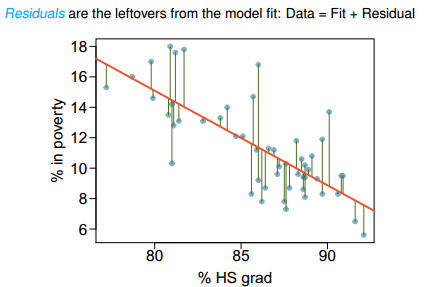
\includegraphics[scale=0.6]{residuals1.png}
    \end{center}
\end{frame}
\begin{frame}{Residuals}
    \begin{center}
        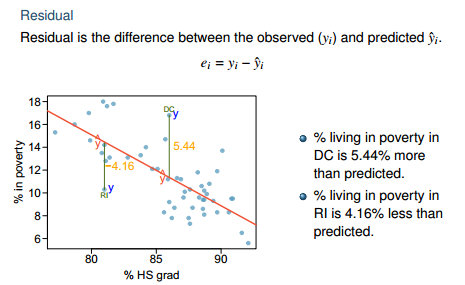
\includegraphics[scale=0.6]{residuals2.png}
    \end{center}
\end{frame}


\begin{frame}{A measure for the best line}
    \begin{center}
        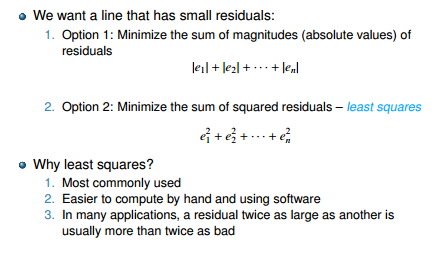
\includegraphics[scale=0.6]{errorMeasures.png}
    \end{center}
\end{frame}
\begin{frame}{Least Squares Line}
    \begin{center}
        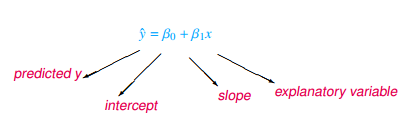
\includegraphics[scale=0.6]{leastSquaresLine.png}
    \end{center}
\end{frame}
\begin{frame}{Prediction}
    \begin{center}
        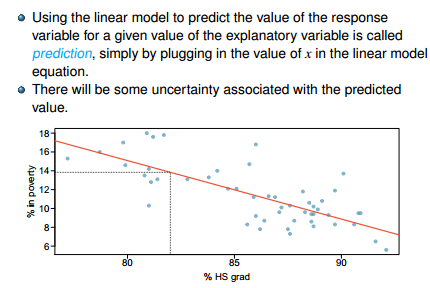
\includegraphics[scale=0.6]{leastSquaresPrediction.png}
    \end{center}
\end{frame}

\begin{frame}{Linear Regression in Higher Dimensions}
    \begin{center}
        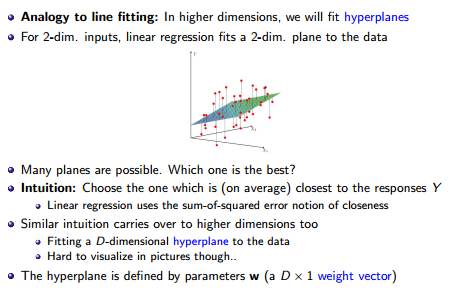
\includegraphics[scale=0.6]{linearRegrHigherD1.png}
    \end{center}
\end{frame}
\begin{frame}{Linear Regression in Higher Dimensions}
    \begin{center}
        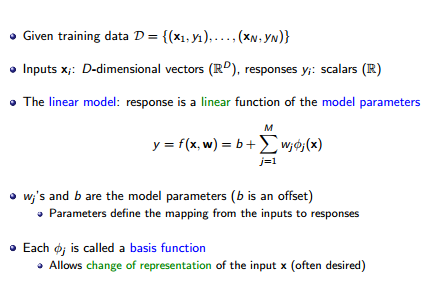
\includegraphics[scale=0.6]{linearRegrHigherD2.png}
    \end{center}
\end{frame}
\begin{frame}{Linear Regression in Higher Dimensions}
    \begin{center}
        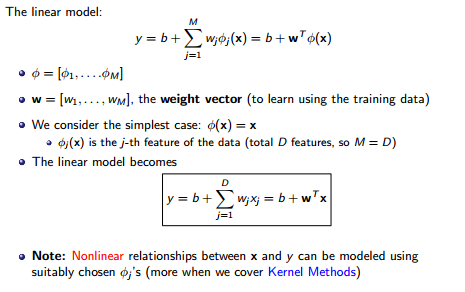
\includegraphics[scale=0.6]{linearRegrHigherD3.png}
    \end{center}
\end{frame}
\begin{frame}{Linear Regression: Objective Function }
    \begin{center}
        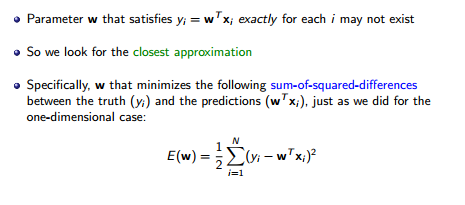
\includegraphics[scale=0.6]{linearRegrObjFn.png}
    \end{center}
\end{frame}
\begin{frame}{Linear Regression: Gradient Descent based Solution}
    \begin{center}
        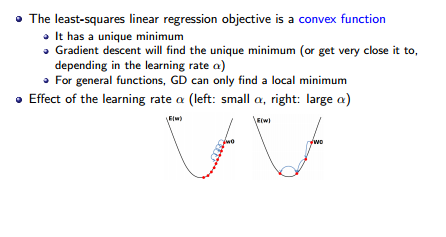
\includegraphics[scale=0.7]{gradientDescent.png}
    \end{center}
\end{frame}

\section{Regression Trees}
\begin{frame}{} 
    \begin{center}
        \thblue{Regression Trees}
    \end{center}
\end{frame}

\begin{frame}{Predicting Baseball salary data}
    
    Salary is color-coded from low (blue, green) to high (yellow,red)
    \begin{center}
        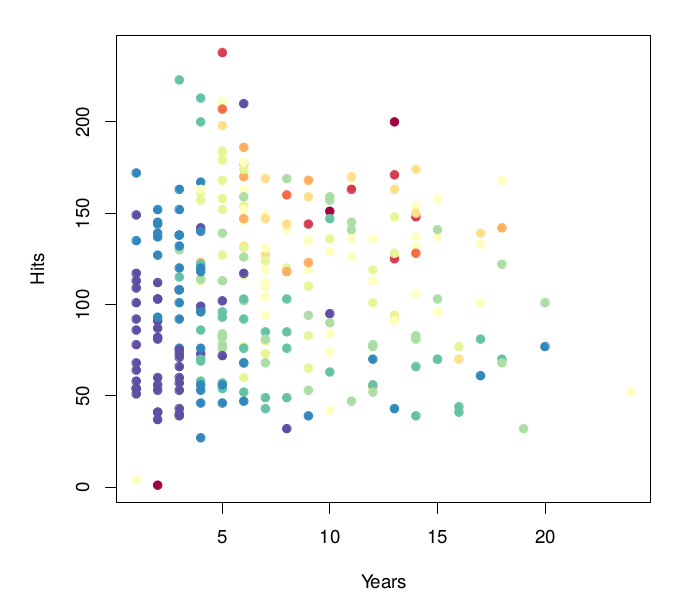
\includegraphics[scale=0.3]{baseballSal1.png}
    \end{center}
\end{frame}
\begin{frame}{Decision tree for Baseball Salary Prediction}
    \begin{center}
        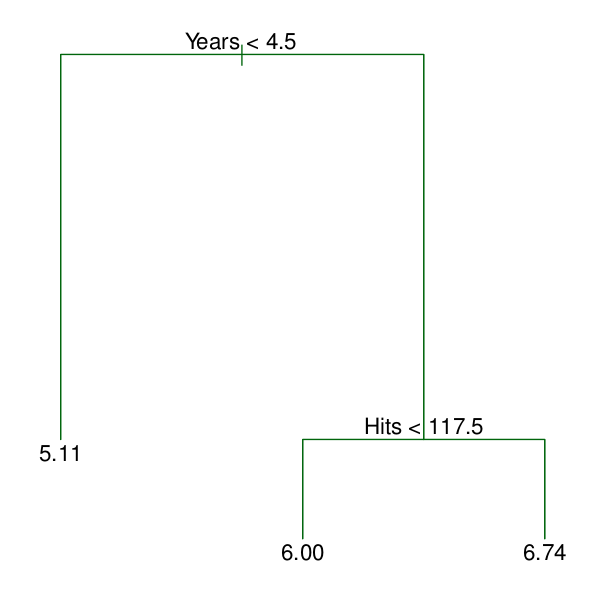
\includegraphics[scale=0.3]{baseballSal2.png}
    \end{center}
\end{frame}
\begin{frame}{Decision tree for Baseball Salary Prediction}
    \begin{center}
        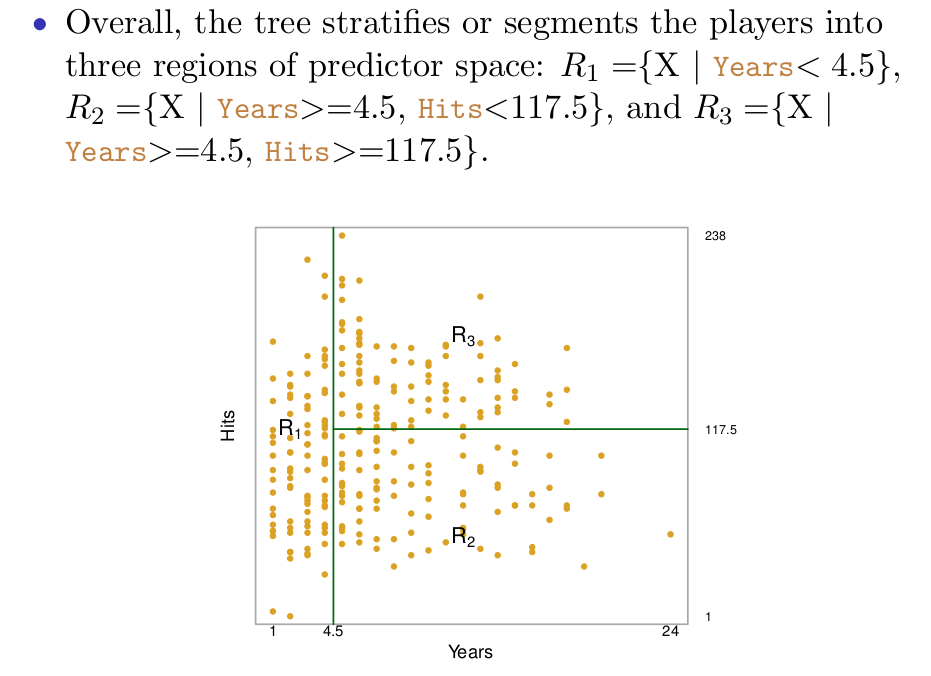
\includegraphics[scale=0.3]{baseballSal3.png}
    \end{center}
\end{frame}

\begin{frame}{Interpreting the Decision Tree}
    \begin{center}
        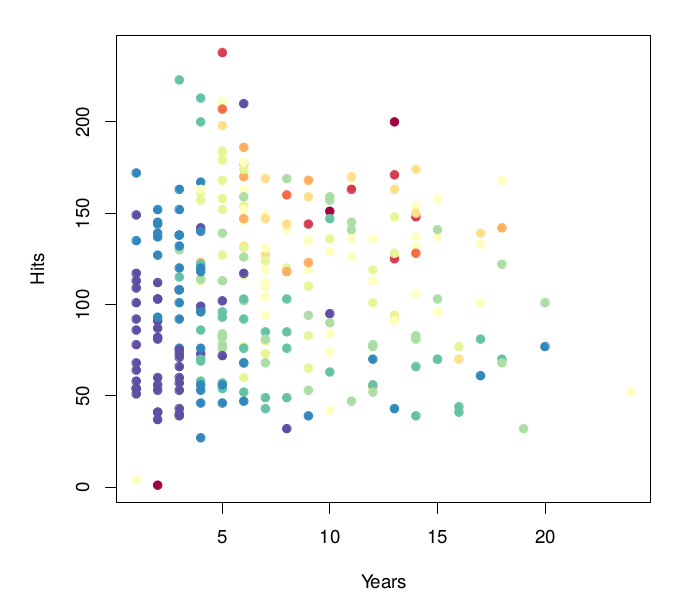
\includegraphics[scale=0.3]{baseballSal1.png}
    \end{center}
\end{frame}
\begin{frame}{Interpreting the Decision Tree}
    \begin{itemize}
        \item Years is the most important factor in determining Salary, and players with less experience earn lower salaries than more experienced players.
        \item Given that a player is less experienced, the number of Hits that he made in the previous year seems to play little role in his Salary .
        \item But among players who have been in the major leagues for five or more years, the number of Hits made in the previous year does affect Salary , and players who made more Hits last year tend to have higher salaries.
        \item Surely an over-simplification, but compared to a regression model, it is easy to display, interpret and explain
    \end{itemize}
\end{frame}

\begin{frame}{High Level Idea}
    \begin{itemize}
        \item {\bf Classification Tree:} Quality of split measured by general ``Impurity measure''
        \item {\bf Regression Tree:} Quality of split measured by ``Squared error''
    \end{itemize}
\end{frame}

\begin{frame}{High Level Idea}
    \begin{itemize}
        \item We divide the feature space into $J$ distinct and non-overlapping regions $R_1, R_2, \ldots, R_J$
        \item For every observation that falls into the region $R_i$, we make same prediction, which is simply the mean of the response values for the training observations in $R_i$
        \item {\bf Objective:} Find boxes $R_1, R_2, \ldots, R_J$  that minimizes Residual Sum of Square (RSS) 
                $$ RSS = \sum_{i=1}^{J} \sum_{j \in R_i} (y_j - \widehat{y_{R_i}})^2$$
            where $\widehat{y_{R_i}}$ is the mean response for the training in the $i$-th box.
    \end{itemize}
\end{frame}


\begin{frame}{Building Regression Trees}
    \begin{itemize}
        \item We first select the feature $X_i$ and the cutpoint $s$ such that splitting the feature space into the regions $\{X|X_i < s\}$ and $\{X|X_i \geq s\}$ leads to the greatest possible reduction in RSS.
        \item Next, we repeat the process, looking for the best attribute and best cutpoint in order to split the data further so as to minimize the RSS within each of the resulting regions.
        \item The process continues until a stopping criterion is reached; for instance, we may continue until no region contains more than five observations.
    \end{itemize}
\end{frame}



\section{Summary}
\begin{frame}{Summary}

\tblue{Major Concepts:}
\begin{itemize}
    \item Geometric interpretation of Classification
    \item Decision trees
\end{itemize}
\end{frame}

\begin{frame}{Slide Material References}
\begin{itemize}
    \item Slides from ISLR book
    \item Slides by Piyush Rai
    \item Slides from OpenIntro Statistics book (\url{http://www.webpages.uidaho.edu/~stevel/251/slides/os2_slides_07.pdf})
    \item See also the footnotes
\end{itemize}
\end{frame}


\end{document}

